%%%%%%%%%%%%%%%%%%%%%%%%%%%%%%%%%%%%%%%%%%%%%%%%%%%%%%%%%%%%%%%
%% CDE THESIS TEMPLATE

% Use this template to produce a standard thesis that meets the CDE master requirements for submission
%
% Originally by Keith A. Gillow (gillow@maths.ox.ac.uk), 1997
% Modified by Sam Evans (sam@samuelevansresearch.org), 2007
% Modified by John McManigle (john@oxfordechoes.com), 2015
% Modified by Ulrik Lyngs (ulrik.lyngs@cs.ox.ac.uk), 2018-, for use with R Markdown
% Modified by Cesar Aybar (csaybar@gmail.com), 2022-, according to CDE format.

% Ulrik Lyngs, 25 Nov 2018: Following John McManigle, broad permissions are granted to use, modify, and distribute this software
% as specified in the MIT License included in this distribution's LICENSE file.
%
% John commented this file extensively, so read through to see how to use the various options.  Remember that in LaTeX,
% any line starting with a % is NOT executed.  Several places below, you have a choice of which line to use
% out of multiple options (eg draft vs final, for PDF vs for binding, etc.)  When you pick one, add a % to the beginning of
% the lines you don't want.


%%%%% PAGE LAYOUT
% The most common choices should be below.  You can also do other things, like replacing "a4paper" with "letterpaper", etc.

% This one formats for two-sided binding (ie left and right pages have mirror margins; blank pages inserted where needed):
%\documentclass[a4paper,twoside]{templates/ociamthesis}
% This one formats for one-sided binding (ie left margin > right margin; no extra blank pages):
%\documentclass[a4paper]{ociamthesis}
% This one formats for PDF output (ie equal margins, no extra blank pages):
%\documentclass[a4paper,nobind]{templates/ociamthesis}

% As you can see from the uncommented line below, oxforddown template uses the a4paper size, 
% and passes in the binding option from the YAML header in index.Rmd:
\documentclass[a4paper, nobind]{templates/cdethesis}


%%%%% ADDING LATEX PACKAGES
% add hyperref package with options from YAML %
\usepackage[pdfpagelabels]{hyperref}
% change the default coloring of links to something sensible
\usepackage{xcolor}

\definecolor{mylinkcolor}{RGB}{0,0,139}
\definecolor{myurlcolor}{RGB}{0,0,139}
\definecolor{mycitecolor}{RGB}{0,33,71}

\hypersetup{
  hidelinks,
  colorlinks,
  linktocpage=true,
  linkcolor=mylinkcolor,
  urlcolor=myurlcolor,
  citecolor=mycitecolor
}



% add float package to allow manual control of figure positioning %
\usepackage{float}

% enable strikethrough
\usepackage[normalem]{ulem}

% use soul package for correction highlighting
\usepackage{color, soul}
\definecolor{correctioncolor}{HTML}{CCCCFF}
\sethlcolor{correctioncolor}
\newcommand{\ctext}[3][RGB]{%
  \begingroup
  \definecolor{hlcolor}{#1}{#2}\sethlcolor{hlcolor}%
  \hl{#3}%
  \endgroup
}
\soulregister\ref7
\soulregister\cite7
\soulregister\autocite7
\soulregister\textcite7
\soulregister\pageref7

%%%%% FIXING / ADDING THINGS THAT'S SPECIAL TO R MARKDOWN'S USE OF LATEX TEMPLATES
% pandoc puts lists in 'tightlist' command when no space between bullet points in Rmd file,
% so we add this command to the template
\providecommand{\tightlist}{%
  \setlength{\itemsep}{0pt}\setlength{\parskip}{0pt}}
 
% UL 1 Dec 2018, fix to include code in shaded environments

% User-included things with header_includes or in_header will appear here
% kableExtra packages will appear here if you use library(kableExtra)
\usepackage{booktabs}
\usepackage{longtable}
\usepackage{array}
\usepackage{multirow}
\usepackage{wrapfig}
\usepackage{float}
\usepackage{colortbl}
\usepackage{pdflscape}
\usepackage{tabu}
\usepackage{threeparttable}
\usepackage{threeparttablex}
\usepackage[normalem]{ulem}
\usepackage{makecell}
\usepackage{xcolor}


%UL set section header spacing
\usepackage{titlesec}
% 
\titlespacing\subsubsection{0pt}{24pt plus 4pt minus 2pt}{0pt plus 2pt minus 2pt}


%UL set whitespace around verbatim environments
\usepackage{etoolbox}
\makeatletter
\preto{\@verbatim}{\topsep=0pt \partopsep=0pt }
\makeatother


%%%%%%% PAGE HEADERS AND FOOTERS %%%%%%%%%
\usepackage{fancyhdr}
\setlength{\headheight}{15pt}
\fancyhf{} % clear the header and footers
\pagestyle{fancy}
\renewcommand{\chaptermark}[1]{\markboth{\thechapter. #1}{\thechapter. #1}}
\renewcommand{\sectionmark}[1]{\markright{\thesection. #1}} 
\renewcommand{\headrulewidth}{0pt}

\fancyhead[LO]{\emph{\leftmark}} 
\fancyhead[RE]{\emph{\rightmark}} 

% UL page number position 
\fancyfoot[C]{\emph{\thepage}} %regular pages
\fancypagestyle{plain}{\fancyhf{}\fancyfoot[C]{\emph{\thepage}}} %chapter pages

% JEM fix header on cleared pages for openright
\def\cleardoublepage{\clearpage\if@twoside \ifodd\c@page\else
   \hbox{}
   \fancyfoot[C]{}
   \newpage
   \if@twocolumn\hbox{}\newpage
   \fi
   \fancyhead[LO]{\emph{\leftmark}} 
   \fancyhead[RE]{\emph{\rightmark}} 
   \fi\fi}


%%%%% SELECT YOUR DRAFT OPTIONS
% This adds a "DRAFT" footer to every normal page.  (The first page of each chapter is not a "normal" page.)

% IP feb 2021: option to include line numbers in PDF

% for line wrapping in code blocks
\usepackage{fvextra}
\DefineVerbatimEnvironment{Highlighting}{Verbatim}{breaklines,commandchars=\\\{\}}

% This highlights (in blue) corrections marked with (for words) \mccorrect{blah} or (for whole
% paragraphs) \begin{mccorrection} . . . \end{mccorrection}.  This can be useful for sending a PDF of
% your corrected thesis to your examiners for review.  Turn it off, and the blue disappears.
\correctionstrue


%%%%% BIBLIOGRAPHY SETUP
% Note that your bibliography will require some tweaking depending on your department, preferred format, etc.
% If you've not used LaTeX before, I recommend reading a little about biblatex/biber and getting started with it.
% If you're already a LaTeX pro and are used to natbib or something, modify as necessary.
% Either way, you'll have to choose and configure an appropriate bibliography format...


\usepackage[style=authoryear, sorting=nyt, backend=biber, maxcitenames=2, useprefix, doi=true, isbn=false, uniquename=false]{biblatex}
\newcommand*{\bibtitle}{Bibliography}

\addbibresource{bibliography/references.bib}


% This makes the bibliography left-aligned (not 'justified') and slightly smaller font.
\renewcommand*{\bibfont}{\raggedright\small}


% Uncomment this if you want equation numbers per section (2.3.12), instead of per chapter (2.18):
%\numberwithin{equation}{subsection}


%%%%% THESIS / TITLE PAGE INFORMATION
% Everybody needs to complete the following:
\title{HOW RELIABLE ARE SENTINEL-2 CLOUD DETECTION ALGORITHMS?:
GLOBAL UNCERTAINTY ESTIMATION WITH GAUSSIAN PROCESSES.}
\author{Cesar Luis Aybar Camacho}
\college{}

% Master's candidates who require the alternate title page (with candidate number and word count)
% must also un-comment and complete the following three lines:

% Uncomment the following line if your degree also includes exams (eg most masters):
%\renewcommand{\submittedtext}{Submitted in partial completion of the}
% Your full degree name.  (But remember that DPhils aren't "in" anything.  They're just DPhils.)
\degree{}
% Term and year of submission, or date if your board requires (eg most masters)
\degreedate{}


%%%%% YOUR OWN PERSONAL MACROS
% This is a good place to dump your own LaTeX macros as they come up.

% To make text superscripts shortcuts
	\renewcommand{\th}{\textsuperscript{th}} % ex: I won 4\th place
	\newcommand{\nd}{\textsuperscript{nd}}
	\renewcommand{\st}{\textsuperscript{st}}
	\newcommand{\rd}{\textsuperscript{rd}}

%%%%% THE ACTUAL DOCUMENT STARTS HERE
\begin{document}

%%%%% CHOOSE YOUR LINE SPACING HERE
% This is the official option.  Use it for your submission copy and library copy:
\setlength{\textbaselineskip}{22pt plus2pt}
% This is closer spacing (about 1.5-spaced) that you might prefer for your personal copies:
%\setlength{\textbaselineskip}{18pt plus2pt minus1pt}

% You can set the spacing here for the roman-numbered pages (acknowledgements, table of contents, etc.)
\setlength{\frontmatterbaselineskip}{17pt plus1pt minus1pt}

% UL: You can set the line and paragraph spacing here for the separate abstract page to be handed in to Examination schools
\setlength{\abstractseparatelineskip}{13pt plus1pt minus1pt}
\setlength{\abstractseparateparskip}{0pt plus 1pt}

% UL: You can set the general paragraph spacing here - I've set it to 2pt (was 0) so
% it's less claustrophobic
\setlength{\parskip}{2pt plus 1pt}

%
% Customise title page
%
\def\crest{{
\includegraphics[width=15cm]{templates/logo.pdf}}}

\renewcommand{\universityfirst}{University of South Brittany, Faculty of Science, Department of Geoinformatics}
\renewcommand{\universitysecond}{Paris Lodron University Salzburg, Faculty of Natural Sciences, Department of Geoinformatics}
\renewcommand{\thesistitlesize}{\fontsize{20pt}{25pt}\selectfont}
\renewcommand{\gapbeforecrest}{25mm}
\renewcommand{\gapaftercrest}{25mm}

\renewcommand{\supervisortextfirst}{Supervisor (University of South Brittany)}
\renewcommand{\supervisornamefirst}{Prof.~Francois Septier}

\renewcommand{\supervisortextsecond}{Co-supervisor (Paris Lodron University Salzburg)}
\renewcommand{\supervisornamesecond}{Prof.~Dirk Tiede}

\renewcommand{\submittedtextfirst}{Specialization track GeoData Science}
\renewcommand{\submittedtextsecond}{Vannes, France, 2022}


% Leave this line alone; it gets things started for the real document.
\setlength{\baselineskip}{\textbaselineskip}


%%%%% CHOOSE YOUR SECTION NUMBERING DEPTH HERE
% You have two choices.  First, how far down are sections numbered?  (Below that, they're named but
% don't get numbers.)  Second, what level of section appears in the table of contents?  These don't have
% to match: you can have numbered sections that don't show up in the ToC, or unnumbered sections that
% do.  Throughout, 0 = chapter; 1 = section; 2 = subsection; 3 = subsubsection, 4 = paragraph...

% The level that gets a number:
\setcounter{secnumdepth}{2}
% The level that shows up in the ToC:
\setcounter{tocdepth}{1}


%%%%% ABSTRACT SEPARATE
% This is used to create the separate, one-page abstract that you are required to hand into the Exam
% Schools.  You can comment it out to generate a PDF for printing or whatnot.

% JEM: Pages are roman numbered from here, though page numbers are invisible until ToC.  This is in
% keeping with most typesetting conventions.
\begin{romanpages}

% Title page is created here
\maketitle

%%%%% DEDICATION
\begin{dedication}
  To Prof.~Bram Leo Willems, who gifted me my first computer ten years ago. This document encapsulates everything I have learned since then.
\end{dedication}

%%%%% ABSTRACT


\renewcommand{\abstracttitle}{Abstract}
\begin{abstract}
	Cloud detection (CD) is one of the most critical metadata filters for searching, selecting, and accessing
 imagery in Earth Observation (EO) platforms. In recent years, the extensive archive of EO datasets
 has boosted the use of data-driven algorithms to improve cloud and cloud-shadow detection. However,
 data-driven algorithms require large manually annotated datasets, which are expensive and time-consuming
 to collect. The first chapter of this diploma thesis introduce CloudSEN12, a new multi-temporal global dataset
 created exploiting different EO datasets offered by the Copernicus program. CloudSEN12 has 49,400 image patches,
 including (1) Sentinel-2 level-1C and level-2A multi-spectral data, (2) Sentinel-1 synthetic aperture radar
 data, (3) auxiliary remote sensing products, (4) different hand-crafted annotations to label the presence
 of clouds and cloud shadows, and (5) the results from eight state-of-the-art cloud detection algorithms. At present,
 CloudSEN12 exceeds all previous efforts in terms of annotation richness, scene variability, metadata complexity,
 control quality, data distribution and size. In the second chapter, cloudSEN12 is used to analize how
 reliable is Sen2COR Sentinel-2 2A cloud mask. The results shows that \ldots{}

 \mbox{}
 \vfill

 \section*{KEYWORDS}

 \noindent cloud detection, deep learning, U-Net, gaussian process, non-stationary. \newline
 Number of pages: 56 \newline
 Number of appendices: 5 \newline
\end{abstract}




%%%%% DECLARATION


\renewcommand{\declarationtitle}{Declaration}
\begin{declaration}
	This thesis has been composed by Cesar Luis Aybar Camacho for the Erasmus
 Mundus Joint Master's Degree Program in Copernicus Master in Digital Earth for the
 academic year 2021/2022 at the Department of Geoinformatics, Faculty of Natural
 Sciences, Paris Lodron University Salzburg, and Department of Geoinformatics, Faculty
 of Science, Southern Brittany University.

 Hereby, I declare that this piece of work is entirely my own, the references cited have
 been acknowledged and the thesis has not been previously submitted to the fulfillment of
 the higher degree.

 \begin{flushright}
 Cesar Aybar \\
 Southern Brittany, France \\
 28 March 2022
 \end{flushright}
\end{declaration}


%%%%% ACKNOWLEDGEMENTS


\begin{acknowledgements}
 	I would like to express my gratitude to my supervisors, Prof.~Francois Septier
  and Prof.~Dirk Tiede, for their constant help and encouragement. From the start
  of the project to the end, your guidance, mentoring, and support cleared the way
  for me to successfully complete this dissertation. The computational requirements
  for this research were partially covered by the Google Cloud Credits Research Grant Program. Besides,
  the Radiant Earth Foundation provides us with a space to store the dataset. This work
  was also partially supported by the Spanish Ministry of Science and Innovation
  (project PID2019-109026RB-I00, ERDF), the Austrian Space Applications Programme
  within the SemantiX project (\#878939, ASAP 16), and the Linux Foundation Grant
  projects (project 21-ISC-1-1). The following R and Python packages
  were used in the course of this investigation and I would like to acknowledge
  their developers: rgee (\cite{Aybar2020}), sf (\cite{Pebesma2018}),
  raster (\cite{hijmans2015package}), stars (\cite{pebesma2020stars}),
  numpy (\cite{harris2020array}), lubridate (\cite{grolemund2011dates}),
  reticulate (\cite{ushey2020reticulate}), dplyr (\cite{wickham2014dplyr}),
  tmap (\cite{tennekes2018tmap}), magick(\cite{ooms2020magick}),
  rgeos (\cite{bivand2017package}) and ggplot2(\cite{wickham2011ggplot2}). Finally,
  I would like to thank B.S. Joselyn Inga and Wendy Espinoza for their work
  reporting manual labeling errors in the quality control phase of the dataset.

  \begin{flushright}
  Cesar Aybar \\
  Southern Brittany, France \\
  28 March 2022
  \end{flushright}
\end{acknowledgements}


%%%%% MINI TABLES
% This lays the groundwork for per-chapter, mini tables of contents.  Comment the following line
% (and remove \minitoc from the chapter files) if you don't want this.  Un-comment either of the
% next two lines if you want a per-chapter list of figures or tables.
  \dominitoc % include a mini table of contents

% This aligns the bottom of the text of each page.  It generally makes things look better.
\flushbottom

% This is where the whole-document ToC appears:
\tableofcontents

\listoffigures
	\mtcaddchapter
  	% \mtcaddchapter is needed when adding a non-chapter (but chapter-like) entity to avoid confusing minitoc

% Uncomment to generate a list of tables:
\listoftables
  \mtcaddchapter
%%%%% LIST OF ABBREVIATIONS
% This example includes a list of abbreviations.  Look at text/abbreviations.tex to see how that file is
% formatted.  The template can handle any kind of list though, so this might be a good place for a
% glossary, etc.
% First parameter can be changed eg to "Glossary" or something.
% Second parameter is the max length of bold terms.
\begin{mclistof}{List of Abbreviations}{3.2cm}

\item[1-D, 2-D]

One- or two-dimensional, referring \textbf{in this thesis} to spatial dimensions in an image.

\item[Otter]

One of the finest of water mammals.

\item[Hedgehog]

Quite a nice prickly friend.

\end{mclistof} 


% The Roman pages, like the Roman Empire, must come to its inevitable close.
\end{romanpages}

%%%%% CHAPTERS
% Add or remove any chapters you'd like here, by file name (excluding '.tex'):
\flushbottom

% all your chapters and appendices will appear here
\begin{savequote}
What am I in the eyes of most people - a nonentity, an eccentric or an
unpleasant person - somebody who has no position in society and never
will have, in short, the lowest of the low. All right, then - even if
that were absolutely true, then I should one day like to show by my work
what such an eccentric, such a nobody, has in his heart.
\qauthor{--- Vincent Van Gogh - 1882}\end{savequote}



\hypertarget{uncertainty-estimation}{%
\chapter{Uncertainty estimation}\label{uncertainty-estimation}}

\minitoc 

\hypertarget{introduction}{%
\section{Introduction}\label{introduction}}

Cloud masking is an essential pre-processing for any application of optical remote sensing imagery. Various coarse-resolution cloud cover datasets (\cite{sassen2008classifying, winker2010calipso, Wilson2016}) estimate the worldwide multi-annual cloud occurrence percentage to be around 0.6 ± 0.2, with hotspots in tropical and subtropical forests. Assuming these products are indicative of Sentinel-2 cloud conditions, we can anticipate that more than half of the pixels will need to be removed, i.e.~masked out, in order to avoid distortions in further analyses. Given that cloud masking can be interpreted as a statistical classification problem, the confusion matrix can be used to distinguish between two distinct types of errors. On the one hand, cloud omission errors (cloud as non-cloud) can lead to inconsistencies in time series of surface reflectance pixels, whereas cloud commission (clear as non-cloud) reduces the number of valid observations and, as a result, the frequency of cloud-free data (\cite{skakun2022cloud}). Cloud masking techniques are aimed to have a balance between commission and omission errors. Over the last three decades, a plethora of cloud masking methods have been presented (\cite{Hagolle2017, Domnich2021, Louis2016, Qiu2019, richter2019atmospheric, jan_wevers_2021_5788067, Lopez-Puigdollers2021, frantz2019force}). These methods can be classified into two main categories: knowledge-driven (KD) and data-driven (DD). While KD emphasizes the use of physical rules formulated on spectral and contextual features, DD is subjected to the exigency of large pixel-level annotation and costly computational requirements to distinguish cloud versus non-cloud regions.

Only a few studies have attempted to compare the various Sentinel-2 cloud masking methods. For instance, \cite{Cilli} compare DD with KD methods by analyzing 135 Sentinel-2 images distributed worldwide. They concluded that DD methods outperform KD methods. According to their experiments, \(10^{4}\) manually labeled pixels are sufficient for train machine learning algorithms to operate accurately cloud masking. Nonetheless, it is well established that DD models are highly dependent on the training dataset (\cite{Lopez-Puigdollers2021}. As a result, the comparison could be unfair, especially if the KD methods have not been as well calibrated to the dataset. \cite{Zekoll2021} compare three KD threshold-based: FMask, ATCOR, and Sen2Cor using a sample-based dataset. The results show that Sen2Cor outperforms the other methods. However, human-made datasets, especially those created by sampling, can be positively skewed if we consider that humans tend to overlook unpleasant information such as cloud borders (ostrich-effect, \cite{Valdez2017}). Using four different datasets, the Cloud Mask Intercomparison eXercise (CMIX) recently compared ten cloud detection algorithms. They suggested that no single algorithm performed better than the others \cite{Skakun2022}. Similar conclusions are found in \cite{tarrio2020comparison} by analyzing 28 images over six Sentinel-2 tiles in Africa and Europe.

In this chapter, we propose to use a novel approach for exploiting the hand-crafted cloud and cloud shadow masking information freely available in cloudSEN12. Unlike previous studies, we intend not only to characterize but also to predict cloud masking uncertainty worldwide. Inspired by deep kernel learning \cite{wilson2016deep}, we explore the use of Gradient boosting Gaussian Processes (GBGP) which combines the structural properties of machine learning architectures with the non-parametric flexibility of kernel methods.

\hypertarget{data}{%
\section{Data}\label{data}}

The basis for Cmask is to predict what the reflectance would be for individual pixels in a Landsat 8 image if cirrus clouds were not present at the time the observations were collected. The basis for those pre- dictions is past observations and the atmospheric conditions, i.e.~the water vapor content, at the time of image acquisition. Therefore, two major inputs were included in this analysis: Integrated Water Vapor (IWV) provided by the second Modern-Era Retrospective analysis for Research and Applications (MERRA-2) and cirrus band time series provided by Landsat 8.

\hypertarget{cloudsen12}{%
\subsection{cloudSEN12}\label{cloudsen12}}

CloudSEN12 is a globally spatio-temporal distributed dataset for cloud and cloud shadow semantic understanding that consists of 49,400 image patches (IP) that are evenly spread throughout all continents except Antarctica (Figure X). Each IP has an average size of 5090 x 5090 meters and contains data from Sentinel-2 optical levels 1C and 2A, Sentinel-1 Synthetic Aperture Radar (SAR), digital elevation model, surface water occurrence, land cover classes, cloud masking results from eight different algorithms and hand-crafted labeling data created using an active learning system \cite{francis_alistair_2020_4172871}. cloudSEN12 offers three different manual annotation types in order to support different deep learning strategies: (i) 10,000 IPs with high-quality pixel-level annotation, (ii) 10,000 IPs with scribble annotation, and (iii) 29,250 unlabeled IPs. Only high-quality IPs are used in this study because of the risk of bias due scene incompleteness in scribble annotation. A detailed description of the CloudSEN12 dataset is given in chapter one.

\hypertarget{sen2cor}{%
\subsection{Sen2Cor}\label{sen2cor}}

Sentinel 2 Correction (\cite{Louis2016}) is a mono-temporal image processor designed for
scene classification and atmospheric correction of Sentinel-2 Level 1C input data. Sen2Cor version 2.8 is the version used in the Sentinel-2 ground segment with L2A processing baseline version 02.12. This processing baseline is the most recurrent version in cloudSEN12 (90\% IPs). Sen2Cor (Figure X) uses a series of spectral reflectance thresholds, ratios, and indices based on bands 1--5, 8, and 10--12 to compute cloud and snow probabilities for each pixel. Besides, it includes a cloud shadow and cirrus detection algorithm. The cloud shadows are estimated by multiplying two probability layers: (1) a geometric probability layer constructed from the
final thick cloud mask, sun position, and cloud height distribution, and (2) radiometric probability layer created from a Kohonen map to detect dark areas. On the other hand, cirrus probabilities are calculated simply by threshold band 10 (1.375 µm). Finally, a series of additional steps to improve the quality of the classification are automatically triggered using a priori information: digital elevation model (DEM) information, ESA CCI Water Bodies Map v4.0 (Lamarche et al., 2017), ESA CCI Land Cover Map v.2.0.7 (2015) and a snow climatology. In this study, SCL classes 8, 9 and 10 were used for cloud, class 3 for cloud shadow and the remaining SCL classes for non-cloud.

\hypertarget{cloud-type-ocurrence}{%
\subsection{Cloud type ocurrence}\label{cloud-type-ocurrence}}

The cloud type ocurrence (CTO) are derived from the CloudSat cloud profiling radar (CPR). This sensor permited for the first time to see cloud vertical structure (Stephens et al.~2008). ClouSat is part from Afternoon Constellation, or A-Train, at a frequency of 94 GHz and an altitude of about 700 km. Since 2011, it only produce daytime-only measurements due to battery malfunction, and in February 2018, the spacecraft systems moved to a lower orbit (C-train) to reduce the risk of collision with the other A-train spacecraft. The track of the satellite overpasses the same location every 16 days and provides a resolution of 1.4 km in cross-track and 1.8 km in along-track. Using the vertical profiles of clouds and precipitation, create an algorithms (\cite{}) to classify clouds according to the Cloud Climatology Project (ISCCP) approach: cumulus (Cu), stratocumulus (Sc), stratus (St), alto- cumulus (Ac), altostratus (As), nimbostratus (Ns), cirrus/ cirrostratus, or deep convective clouds. This information is storage in the 2B-CLDCLASS product. Particularly, in this study, we make use of the 3S-RMCP product of CloudSat level 3 observations. This product collocated 2B-CLDCLASS measurements in a 2.5°x2.5° grid. Based on this dataset, we constructed cloud type occurrence at 1° spatial
resolution. The TPR data used corresponds to the 2007--2016 period, the cloud type ocurrence were smoothed from 2.5° to 1° using cubic spline interpolation. We aggregathed the ISCCP classification into three classes accordin to the table x.

\hypertarget{modis}{%
\subsection{MODIS}\label{modis}}

\hypertarget{methodology}{%
\section{Methodology}\label{methodology}}

This study aims to create a model that predicts cloud masking error in
a 1° x 1° worldwide grid system \(y^*\) from a set of predictors \(x^*\). The regression model \(\mathbf{f}\) is trained using a dataset, \(\mathcal{D} = \{x_i, y_i\}^{N}_{i=1}\) with \(x_i\) and \(y_i \in \mathbb{R}\). The segment \(x_i\) represents a vector of \(1 \times m\) predictors (Table X), \(y_i\) is the metric error values (see section \ref{section:metrics}) determined from comparing cloudSEN12 and Sen2Cor cloud masking results, and \(N\) the number of observations set as 10000. Only high-quality IPs are used in this study because of the risk of bias due to scene incompleteness in scribble annotation. A detailed description of the CloudSEN12 dataset is given in chapter one. We propose the use of a deep kernel learning (DKL) regression. It combines deep neural networks (DNN) with standard gaussian process regression (GP). While ANN captures the non-stationary and hierarchical structure, GP permits the estimation of their uncertainty considering the local autocorrelation of the observations. \cite{rasmussen2003gaussian} provide a detail description of GP. The standard GP, DKL, and the approach used to create worldwide cloud error predictions are briefly reviewed in the following sections.

\hypertarget{gaussian-process-regresion}{%
\subsection{Gaussian process regresion}\label{gaussian-process-regresion}}

Standard Gaussian Process Regression (GP) models is a expressive probabilistic model in which both training and testing data points are regarded samples of a joint multivariate normal distribution (\cite{williams2006gaussian}). As other regression models, a GP model is formed by noisy variables of the true underlying function \(\mathbf{f}\) that projects the vector space \(X\) into real-valued targets \(y\), i.e.~\(y = f(\mathbf{x}) + \epsilon\). The element \(\epsilon\) represents the noise variables with \(\mathcal{N}(0, \sigma^{2})\). In a GP model we assume that all the finite dimensional distributions \(f(\mathbf{x})\) are normally distributed with \(\mu\) as a mean and \(K_{XX}|\gamma\) as the prior covariance matrix. The covariance (kernel) matrix regulates the smoothness of GPs and its values are implicitly dependent on the kernel hyperparameters \(\gamma\). In this specific case, the estimation of \(f(\mathbf{x})\) can be expressed given by:

\begin{equation}
\begin{aligned}
\mathbf{f} = f(\mathbf{x}) = [f(x_1), ...., f(x_m)]^\top & \sim 
\mathcal{GP}\left(
  \mu, K_{XX}|\gamma\right
) \\
\end{aligned} \label{eq:1}
\end{equation}

Conditioning the joint normal distribution by the output values at the training points
(\(X\) and \(\mathbf{y}\)), the posterior distribution of the output values \(f(\mathbf{x}_{*})\) at the test data point \(X_*\) can be inferred as:

\begin{equation}
\begin{aligned}
f(\mathbf{x}_{*}) \mid X_{*}, X, \mathbf{y}, \boldsymbol{\gamma}, \sigma^{2} \sim \mathcal{N}(\mu^{*}, \Sigma^{*}), \\
\mu^{*} = \mu_{X_*} + K_{X_*X}\widehat{K}_{XX}^{-1}\mathbf{y}, \\
\Sigma^{*} = K_{X_*X_*} - K_{X_*X}\widehat{K}_{XX}^{-1}K_{XX_*}
\end{aligned} \label{eq:2}
\end{equation}

A hat denotes an added diagonal, i.e.~\(\widehat{K}_{XX} = K_{XX} + + \sigma^{2}I\). \(\mu^{*}\) and \(\Sigma^{*}\) are the posterior mean and covariance matrix respectively. The matrices of the form \(K_{X_iX_j}\) denote cross-covariances between the train (\(X\)) and test (\(X_*\)) vector spaces. The hyperparameters \(\lambda\) of the kernel are usually learned directly by minimizing the negative log marginal likelihood \(\mathcal{L}(\theta)\) with respect to training observations:

\begin{equation}
\begin{aligned}
\mathcal{L} = - \log p(\mathbf{y} \mid \gamma, X) \propto \mathbf{y}^{\top} \widehat{K}_{XX}^{-1} \mathbf{y} + \log \left|\widehat{K}_{X X}\right|, \\
\frac{\partial \mathcal{L}}{\partial \theta} = \mathbf{y}^{\top} \widehat{K}_{XX} \frac{\partial \widehat{K}_{X X}^{-1}}{\partial \theta} \widehat{K}_{X X} \mathbf{y}-\operatorname{tr}\left\{\widehat{K}_{X X}^{-1} \frac{\partial \widehat{K}_{XX}}{\partial \theta}\right\}
\label{eq:3}
\end{aligned}
\end{equation}

The main bottleneck for kernel learning is solve the linear system \(\widehat{K}_{XX}^{-1}y\) in equation \ref{eq:3}. The standard approach is to compute the Cholesky decomposition of the matrix \(\widehat{K}_{XX}^{-1}\). The Cholesky decomposition's core algorithm
uses a divide-and-conquer approach that is inefficient on GPU acceleration (\cite{krishnamoorthy2013matrix}). Furthermore, it requires \(\mathcal{O}(n^{3})\) computation and \(\mathcal{O}(n2)\) storage for GP inference and kernel learning (\cite{rasmussen2003gaussian}). To address the above challenges, several approaches to scaling up GP inference have been proposed (\cite{gardner2018gpytorch, cunningham2008fast, dong2017scalable, bach2013sharp, wilson2015thoughts}). In this paper, we address the GP inference issue by using the Blackbox Matrix-Matrix multiplication inference (BBMM, \cite{gardner2018gpytorch}). BBMM use preconditioned batched conjugate gradients to solve linear systems, reducing the asymptotic time complexity of GP inference from \(\mathcal{O}(n^{3})\) to \(\mathcal{O}(n^{2})\). Besides, it overcomes memory constraints by divvying the kernel matrix to perform matrix-vector multiplication (MVM, \cite{demmel1997applied}) without having to explicitly construct the kernel matrix, reducing the memory requirement to \(\mathcal{O}(n)\). Finally, BBMM parallelize partitioned MVMs across multiple core, enabling a better use of GPU hardware in comparison to the Cholesky factorization.

\hypertarget{deep-kernel-learning}{%
\subsection{Deep kernel learning}\label{deep-kernel-learning}}

DKL is a probabilistic deep network that simultaneously learns a feature
extractor and a Gaussian process on the feature space (cite). The network's
structure is depicted in Figure X. The deep non-linear feature extractor
\(\mathbf{h(x,w)}\), parametrized by weights \(\mathbf{w}\), is applied to the
observed input variable \(\mathbf{x}\). Next, the DNN outputs are modeled using
\(\mathcal{GP}\) by:

\begin{equation}
f(\mathbf{x}) \sim \mathcal{GP}(
    \mu(\mathbf{h_w(x)}),
    k_{\gamma}(\mathbf{h_w(x)}, \mathbf{h_w({x}')})
)
\end{equation}

All parameters of the model, including neural network weights \(\mathbf{w}\) and kernel parameters \(\mathbf{\gamma}\), are optimized end-to-end via backpropagation to minimize the
negative log marginal likelihood (equation \ref{eq:3}).

\begin{figure}[!h]
    \centering
    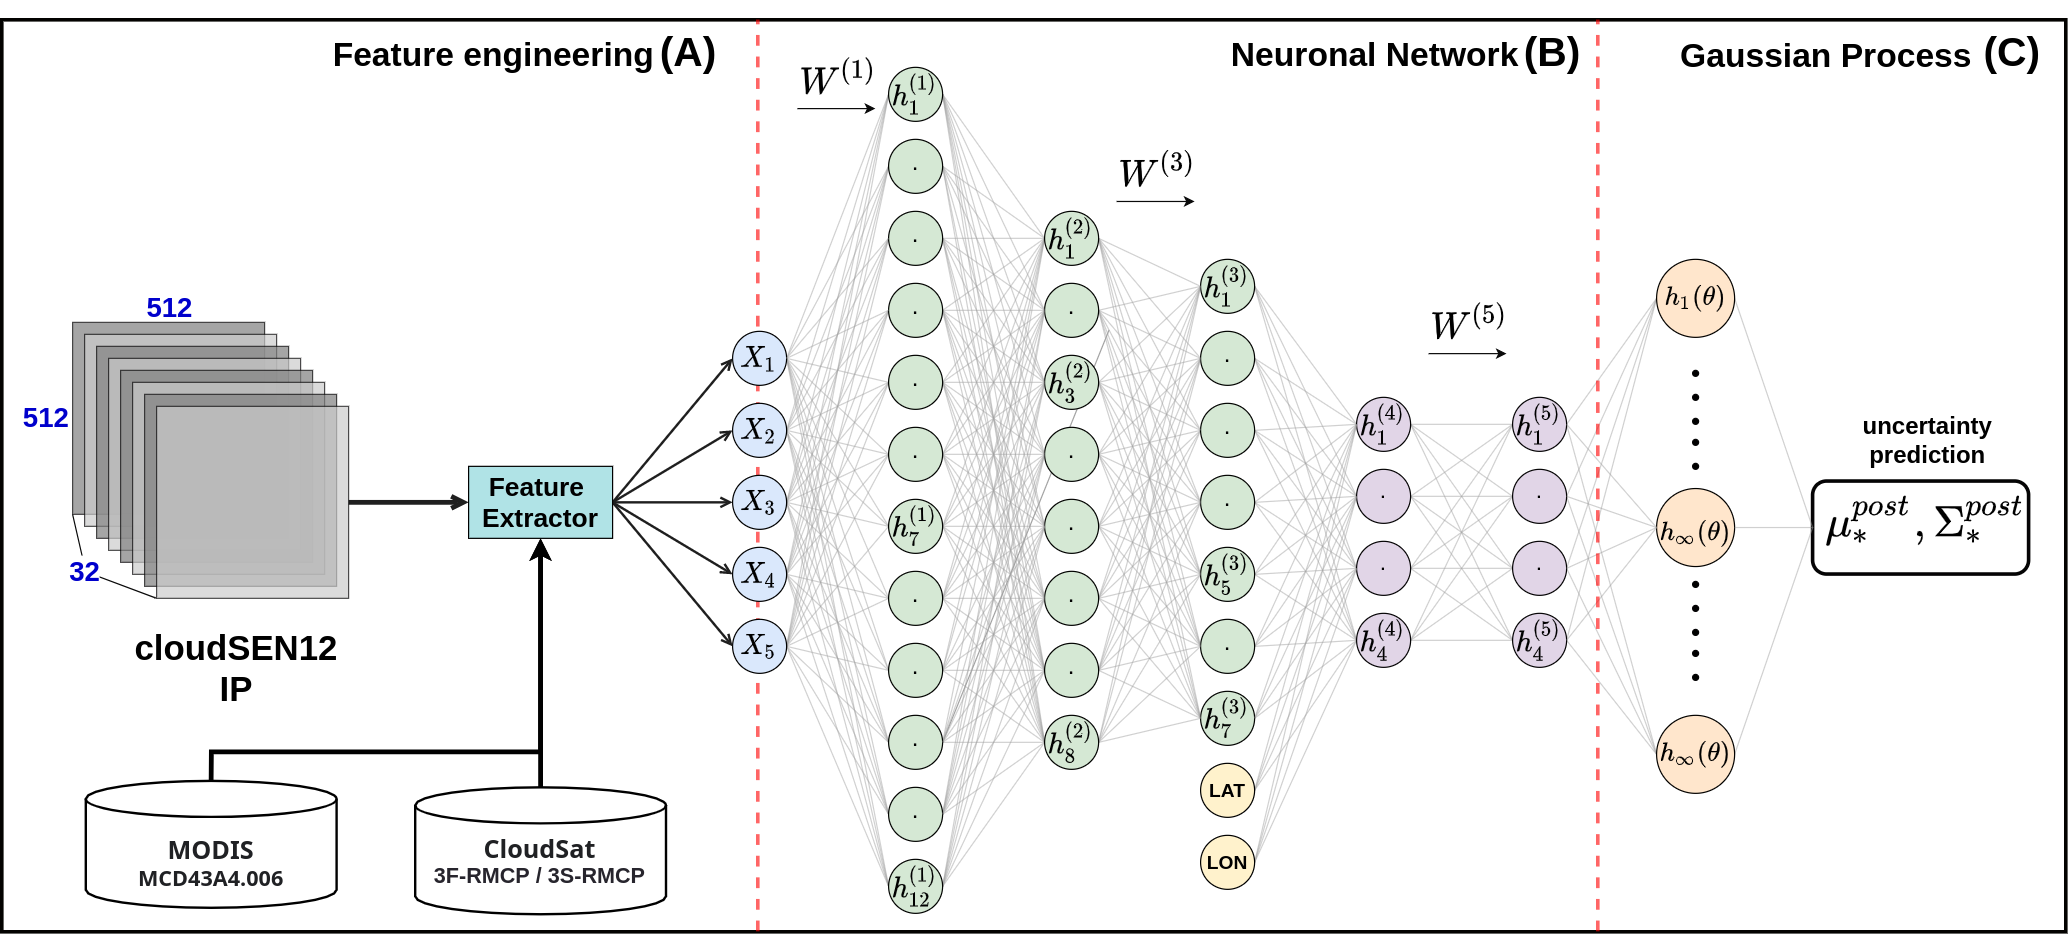
\includegraphics[width=1\linewidth]{figures/chapter02/figure02.png}
    \caption{Number of hand-crafted pixel annotations between different cloud detection datasets. All the labeled pixels in the CloudSEN12 no-annotation group come from cloud-free IPs.}
    \label{fig:figure02}
\end{figure}

\hypertarget{model-set-up-and-training}{%
\subsection{Model set-up and training}\label{model-set-up-and-training}}

For our deep kernel learning model, we used deep neural networks which produce
C-dimensional top-level features. Here C is the number of classes. We place a Gaussian process on each dimension of these features. We used RBF base kernels. The additive GP layer is then followed by a linear mixing layer A R C×C . We initialized A to be an identity matrix, and optimized in the joint learning procedure to recover cross-dimension correlations from data.
We first train a deep neural network using SGD with the softmax loss objective, and rectified linear activation functions. After the neural network has been pre-trained, we fit an additive KISS-GP layer, followed by a linear mixing layer, using the top-level features of the deep network as inputs. Using this pre-training initialization, our joint SV-DKL model of section 3 is then trained through the stochastic variational method of section 4 which jointly optimizes all the hyperparameters of the deep kernel (including all network weights), as well as the variational parameters, by backpropagating derivatives through the proposed marginal likelihood lower bound of the additive Gaussian process in section 4. In all experiments, we use a relatively large mini-batch size (specified according to the full data size), enabled by the proposed structure exploiting variational inference procedures. We achieve good performance setting the number of samples T = 1 in Eq. 4 for expectation estimation in variational inference, which provides additional confirmation for a similar observation in {[}14{]}.

\hypertarget{model-metrics}{%
\subsection{Model metrics}\label{model-metrics}}

\label{section:metrics}

\hypertarget{model-predictions}{%
\subsection{Model predictions}\label{model-predictions}}

\hypertarget{experimental-results}{%
\section{Experimental results}\label{experimental-results}}

\hypertarget{discussion}{%
\section{Discussion}\label{discussion}}

dsada

\hypertarget{conclusion}{%
\section{Conclusion}\label{conclusion}}

dsada

\begin{savequote}
I may not have lived long, but I am certain of one thing. If there is a
type of person capable of changing something, it is someone who is
willing to sacrifice what he values most!. He is the type of person who,
in order to confront a monster, is capable of losing his own humanity. A
person who is unable to make a sacrifice may be unable to change
anything!
\qauthor{--- Armin Arlelt}\end{savequote}



\hypertarget{conclusion-1}{%
\chapter*{Conclusion}\label{conclusion-1}}
\addcontentsline{toc}{chapter}{Conclusion}

If we don't want Conclusion to have a chapter number next to it, we can add the \texttt{\{-\}} attribute.

\hypertarget{more-info}{%
\section*{More info}\label{more-info}}
\addcontentsline{toc}{section}{More info}

And here's some other random info:
the first paragraph after a chapter title or section head \emph{shouldn't be} indented, because indents are to tell the reader that you're starting a new paragraph.
Since that's obvious after a chapter or section title, proper typesetting doesn't add an indent there.

This paragraph, by contrast, \emph{will} be indented as it should because it is not the first one after the `More info' heading.
All hail LaTeX. (If you're reading the HTML version, you won't see any indentation - have a look at the PDF version to understand what in the earth this section is babbling on about).

\startappendices

\hypertarget{appendix---code}{%
\chapter{Appendix - Code}\label{appendix---code}}

This first appendix includes the non-stationary gaussian processes in Gpytorch:

\textbf{In 02-rmd-basics-code.Rmd}

\textbf{And here's another one from the same chapter, i.e.~Chapter \ref{code}:}

\hypertarget{appendix---figures}{%
\chapter{Appendix - Figures}\label{appendix---figures}}

\setcounter{figure}{0}
\makeatletter 
\renewcommand{\thefigure}{S\@arabic\c@figure}
\makeatother

\begin{figure}[!h]
    \centering
    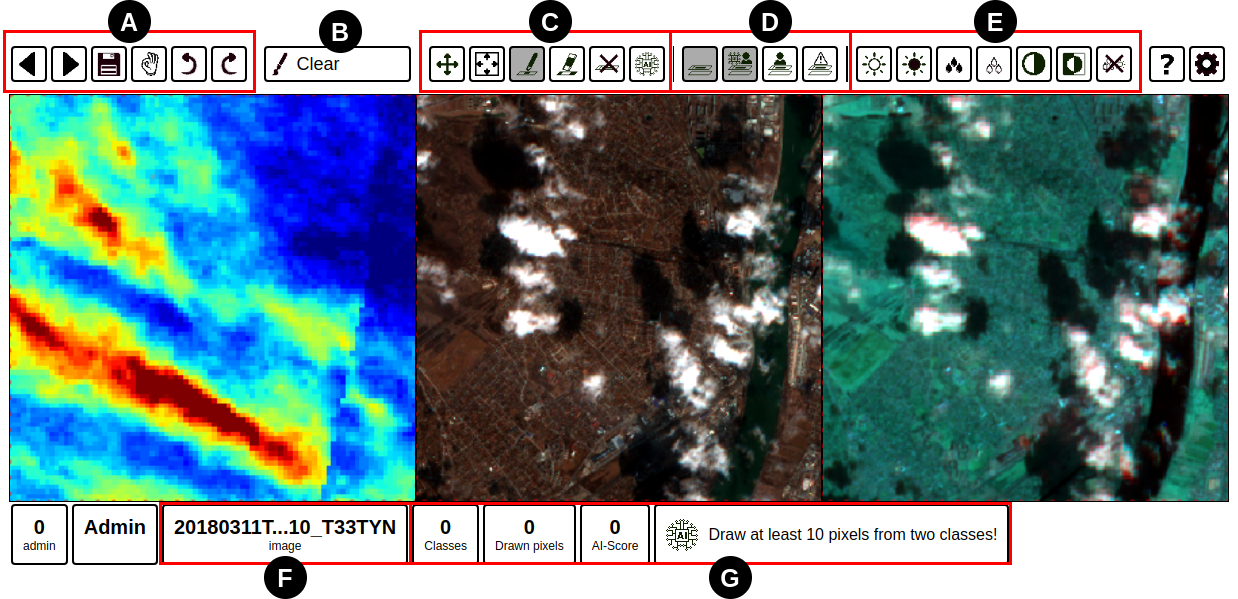
\includegraphics[width=1\linewidth]{figures/extra/figureS2.png}
    \caption{XXXX}
    \label{fig:figureS02}
\end{figure}

\begin{figure}[!h]
    \centering
    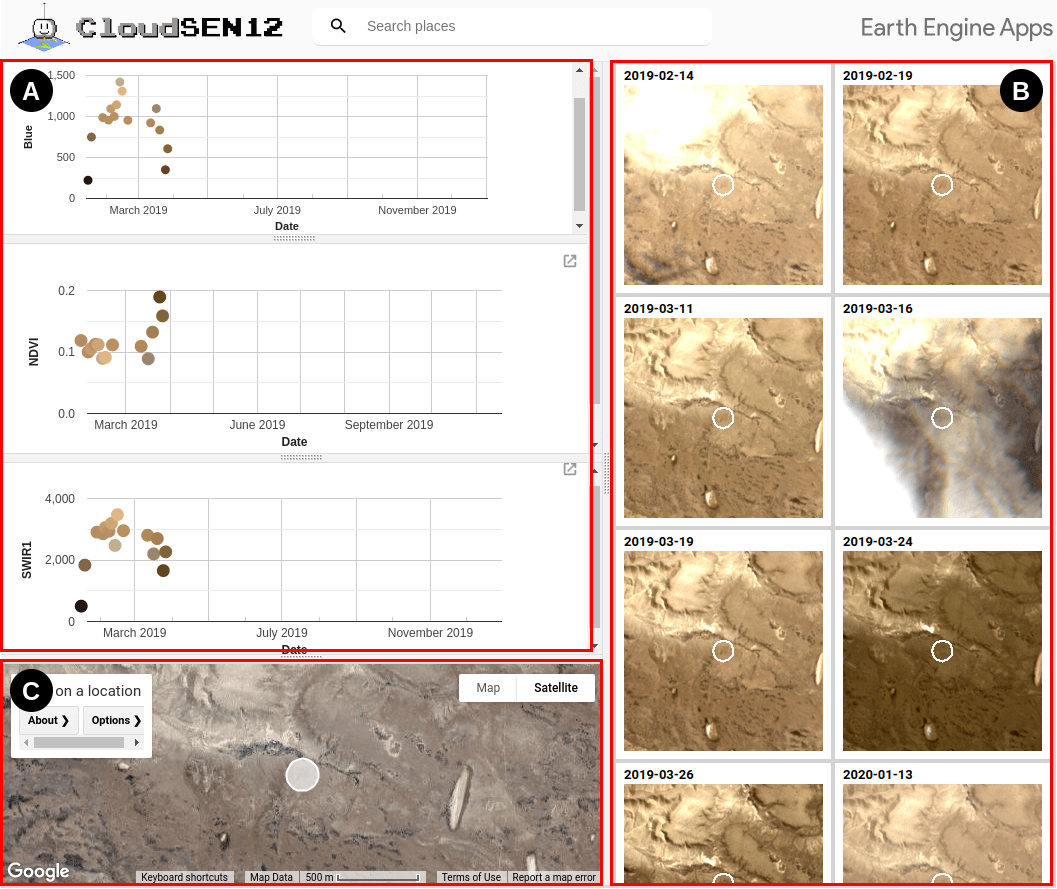
\includegraphics[width=1\linewidth]{figures/extra/figureS3.png}
    \caption{XXXX}
    \label{fig:figureS03}
\end{figure}


%%%%% REFERENCES
\setlength{\baselineskip}{0pt} % JEM: Single-space References

{\renewcommand*\MakeUppercase[1]{#1}%
\printbibliography[heading=bibintoc,title={\bibtitle}]}


\end{document}
